\documentclass[aspectratio=169,10pt]{beamer}
\usetheme{Madrid}
\usecolortheme{default}

\usepackage[utf8]{inputenc}
\usepackage[T1]{fontenc}
\usepackage{amsmath,amssymb}
\usepackage{booktabs}
\usepackage{graphicx}
\usepackage{listings}
\usepackage{hyperref}

\definecolor{unibblue}{RGB}{0,51,102}
\definecolor{unibgold}{RGB}{212,175,55}
\definecolor{unibgreen}{RGB}{0,128,0}
\definecolor{codebg}{RGB}{244,247,251}

\setbeamercolor{structure}{fg=unibblue}
\setbeamercolor{palette primary}{bg=unibblue,fg=white}
\setbeamercolor{palette secondary}{bg=unibblue!85,fg=white}
\setbeamercolor{palette tertiary}{bg=unibblue!70,fg=white}
\setbeamercolor{block title}{bg=unibblue!90,fg=white}
\setbeamercolor{block body}{bg=unibblue!8,fg=black}
\setbeamercolor{alertblock title}{bg=unibgold!90,fg=black}
\setbeamercolor{alertblock body}{bg=unibgold!14,fg=black}
\setbeamercolor{exampleblock title}{bg=unibgreen!85,fg=white}
\setbeamercolor{exampleblock body}{bg=unibgreen!8,fg=black}

\lstset{
  language=Python,
  basicstyle=\ttfamily\scriptsize,
  backgroundcolor=\color{codebg},
  frame=single,
  rulecolor=\color{unibblue!35},
  keywordstyle=\color{unibblue}\bfseries,
  commentstyle=\color{unibgreen!80!black}\itshape,
  showstringspaces=false,
  breaklines=true
}

\title[Aliran Daya Python — Modul 3]{Analisis Aliran Daya Menggunakan Python}
\subtitle{Modul 3: Otomasi \& Skala Industri Menggunakan \texttt{pandapower}}
\author[Novalio Daratha]{Novalio Daratha\\Program Studi Teknik Elektro, Universitas Bengkulu}
\date{Workshop Teknis Intensif (32 JP) — 2026}

\begin{document}

\begin{frame}
  \titlepage
\end{frame}

\begin{frame}{Agenda Modul 3 (8 JP)}
  \tableofcontents
\end{frame}

\section{Arsitektur Data \texttt{pandapowerNet}}

\begin{frame}{Transisi dari \textit{From-Scratch} ke Pustaka Kelas Industri}
  \begin{columns}[T]
    \begin{column}{0.54\textwidth}
      \textbf{Struktur Tabel \texttt{pandas.DataFrame}:}
      \vspace{0.15cm}
      \scriptsize
      \begin{tabular}{@{}lll@{}}
        \toprule
        \textbf{Tabel Input} & \textbf{Kolom Utama} & \textbf{Tabel Hasil} \\
        \midrule
        \texttt{net.bus} & \texttt{vn\_kv, min/max\_vm\_pu} & \texttt{res\_bus} \\
        \texttt{net.ext\_grid} & \texttt{vm\_pu, va\_degree} & \texttt{res\_ext\_grid} \\
        \texttt{net.gen} & \texttt{p\_mw, vm\_pu, min/max\_q} & \texttt{res\_gen} \\
        \texttt{net.load/shunt} & \texttt{p\_mw, q\_mvar} & \texttt{res\_load/shunt} \\
        \texttt{net.line} & \texttt{r/x\_ohm\_per\_km, c\_nf, max\_i\_ka} & \texttt{res\_line} \\
        \texttt{net.trafo} & \texttt{sn\_mva, vk\%, vkr\%, tap\_*} & \texttt{res\_trafo} \\
        \bottomrule
      \end{tabular}
    \end{column}
    \begin{column}{0.44\textwidth}
      \begin{alertblock}{Dua Konvensi Penting Validasi Silang}
        \begin{enumerate}
          \item \texttt{res\_bus} memakai \textbf{konvensi beban positif} (daya keluar bus $> 0$) dan mengikutkan daya elemen \texttt{net.shunt}.
          \item \texttt{res\_line.loading\_percent} memakai rasio \textbf{arus} ($|I|/I_{\max}$), bukan daya semu ($|S|/S_{\text{rate}}$).
        \end{enumerate}
      \end{alertblock}
    \end{column}
  \end{columns}
\end{frame}

\section{Konversi Parameter Per-Unit ke Satuan SI}

\begin{frame}[fragile]{Pemetaan Parameter Per-Unit MATPOWER $\to$ Fisik SI}
  \begin{block}{Transformasi Impedansi, Kapasitansi \& Tegangan Hubung Singkat}
    \[
      r_{\Omega} = r_{\text{pu}} Z_{\text{base}},\quad
      x_{\Omega} = x_{\text{pu}} Z_{\text{base}},\quad
      c\,[\text{nF}] = \frac{b_{\text{pu}}}{2\pi f Z_{\text{base}}}\times 10^{9},\quad
      v_k\% = 100 |z_{\text{pu}}|\frac{S_n}{S_{\text{base}}}
    \]
  \end{block}
\begin{lstlisting}
import pandapower as pp, pandapower.converter as pc
from ybus import get_ieee14_case

case = get_ieee14_case()
ppc = {"version": "2", "baseMVA": case["baseMVA"],
       "bus": case["bus"].copy(), "gen": case["gen"].copy(), "branch": case["branch"].copy()}
net = pc.from_ppc(ppc, f_hz=60.0, validate_conversion=False)
pp.runpp(net, algorithm="nr", init="flat", tolerance_mva=1e-8)
\end{lstlisting}
  \begin{exampleblock}{Validasi Presisi Mesin (Modul 2 vs Modul 3)}
    Deviasi maksimum terhadap solver \textit{from-scratch}: $\max ||V_{\text{NR}}| - |V_{\text{pp}}|| = \mathbf{4{,}44 \times 10^{-16}\text{ p.u.}}$
  \end{exampleblock}
\end{frame}

\section{Evaluasi Profil Tegangan \& Audit Rugi-Rugi}

\begin{frame}{Profil Tegangan 14-Bus \& Distribusi Rugi Transmisi}
  \begin{center}
    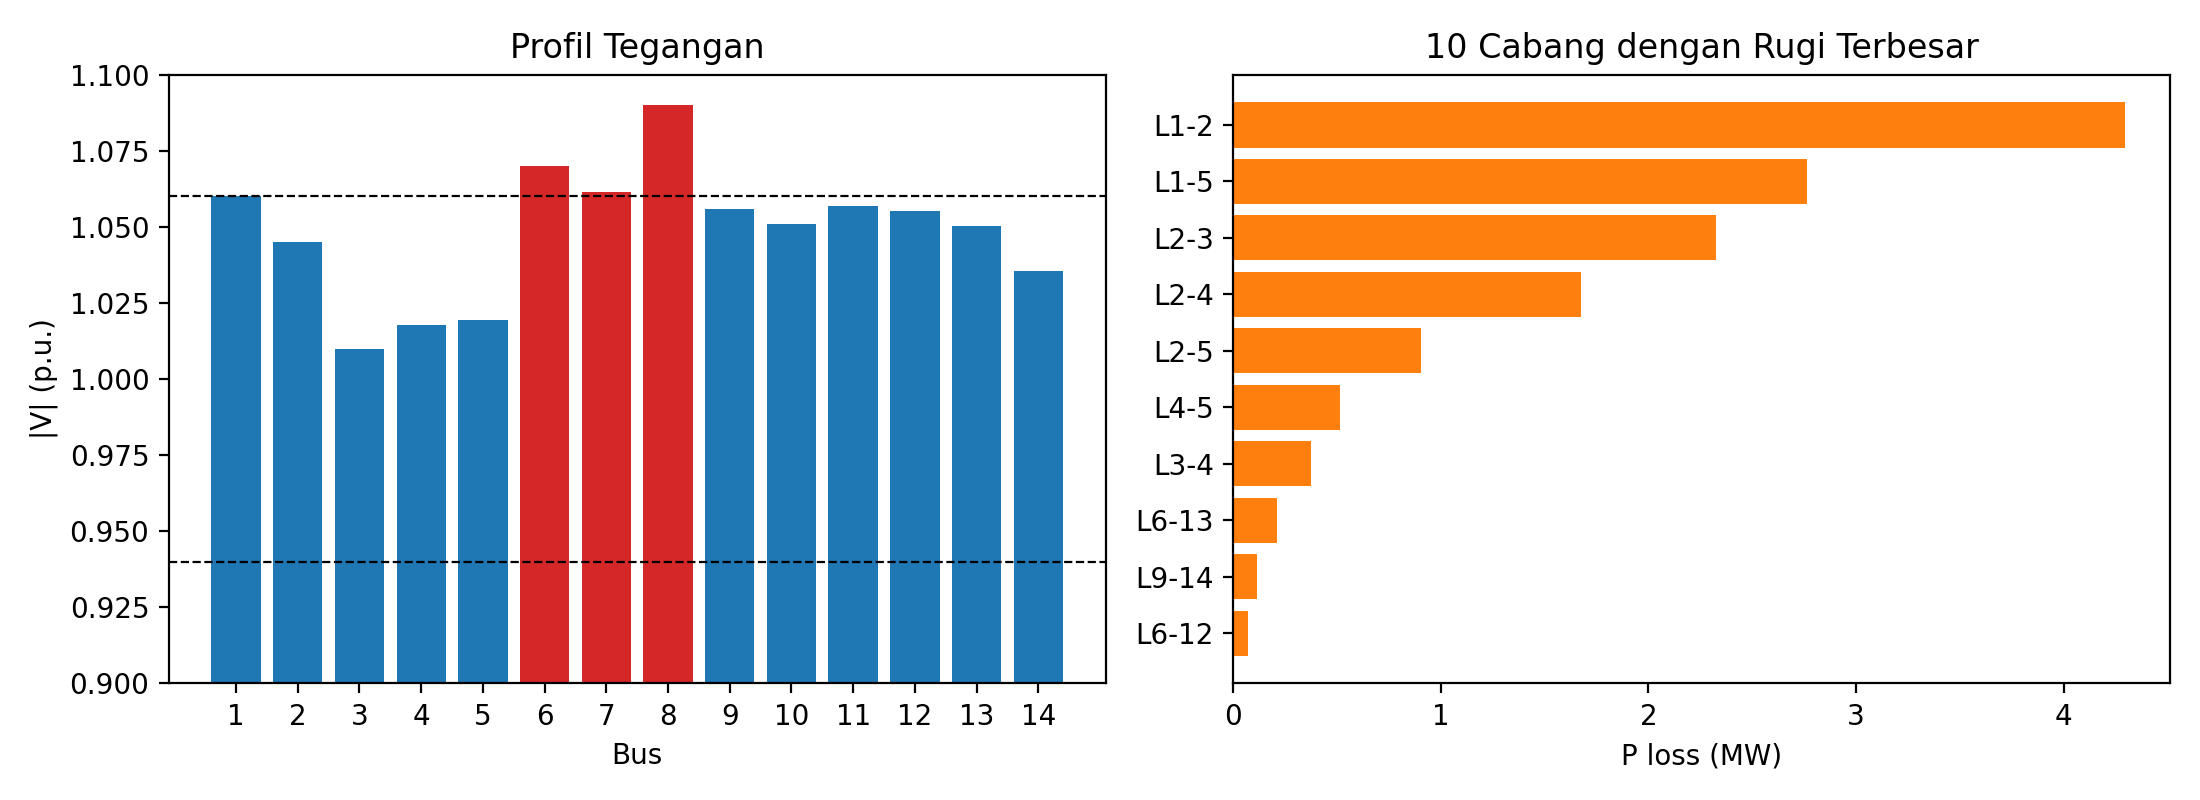
\includegraphics[width=0.95\textwidth]{../figures/profil_tegangan_rugi.png}
  \end{center}
  \vspace{-0.15cm}
  \begin{columns}[T]
    \begin{column}{0.49\textwidth}
      \begin{block}{Audit Neraca Daya (Beban 259,0 MW)}
        \scriptsize
        Rugi aktif total: \textbf{13,393 MW} ($5{,}17\%$ beban) $+ j30{,}122\text{ MVAr}$.\\
        Top 3 penyumbang rugi: \texttt{L1-2} (4,30 MW / 32,1\%), \texttt{L1-5} (2,76 MW), \texttt{L2-3} (2,32 MW).
      \end{block}
    \end{column}
    \begin{column}{0.49\textwidth}
      \begin{exampleblock}{Tugas Lab 3.5: Sapuan Beban 0,6--1,6$\times$}
        \scriptsize
        Bangun fungsi parametris \texttt{scenario(net, load\_factor)} untuk memetakan kurva $V_{\min}$ dan $P_{\text{loss}}$ serta titik pelanggaran pertama!
      \end{exampleblock}
    \end{column}
  \end{columns}
\end{frame}

\begin{frame}{Terima Kasih — Lanjut ke Modul 4}
  \begin{center}
    \vspace{0.8cm}
    {\Large \textbf{Terima Kasih}}\\
    \vspace{0.4cm}
    {\large Sesi Tanya Jawab \& Praktikum \texttt{python3 kode/modul3\_pandapower.py}}\\
    \vspace{1.2cm}
    Novalio Daratha\\
    Program Studi Teknik Elektro, Universitas Bengkulu\\
    \texttt{https://ndaratha.my.id/w-pf/}
  \end{center}
\end{frame}

\end{document}
